\documentclass[UTF8]{ctexart}
\usepackage{geometry}
\usepackage[backend=biber, style=authoryear]{biblatex} % 示例配置
\addbibresource{references.bib} % 替换为你的参考文献文件
\geometry{margin=1.5cm, vmargin={0pt,1cm}}
\setlength{\topmargin}{-1cm}
\setlength{\paperheight}{29.7cm}
\setlength{\textheight}{25.3cm}

% useful packages.
\usepackage{amsfonts}
\usepackage{amsmath}
\usepackage{amssymb}
\usepackage{amsthm}
\usepackage{enumerate}
\usepackage{graphicx}
\usepackage{multicol}
\usepackage{fancyhdr}
\usepackage{layout}
\usepackage{listings}
\usepackage{xcolor}
\lstset{language=C++}
\setlength{\headheight}{13pt}  % 增加头部高度
\usepackage{float, caption}

% Listings setting for code formatting
\lstset{
    basicstyle=\ttfamily,
    keywordstyle=\color{blue},
    commentstyle=\color{gray},
    stringstyle=\color{red},
    breaklines=true,
    frame=single,
    numbers=left,
    numberstyle=\tiny,
    stepnumber=1,
    tabsize=4
}

% some common commands
\newcommand{\dif}{\mathrm{d}}
\newcommand{\avg}[1]{\left\langle #1 \right\rangle}
\newcommand{\difFrac}[2]{\frac{\dif #1}{\dif #2}}
\newcommand{\pdfFrac}[2]{\frac{\partial #1}{\partial #2}}
\newcommand{\OFL}{\mathrm{OFL}}
\newcommand{\UFL}{\mathrm{UFL}}
\newcommand{\fl}{\mathrm{fl}}
\newcommand{\op}{\odot}
\newcommand{\Eabs}{E_{\mathrm{abs}}}
\newcommand{\Erel}{E_{\mathrm{rel}}}

\begin{document}

\pagestyle{fancy}
\fancyhead{}
\lhead{陈梓锐}
\chead{22435036}
\rhead{\today}


%\begin{abstract}
 %   The abstract is not necessary for the theoretical homework, 
   % but for the programming project, 
    %you are encouraged to write one.      
%\end{abstract}

% ============================================

\subsection*{Exercise 9.5}
因为$\|AB\|_2 \leq \|A\|_2 \times \|B\|_2, e = A^{-1}r, b = Ax \Rightarrow \|e\|_2 \leq \|A^{-1}\|_2 \times \|r\|_2
, \|b\|_2 \leq \|A\|_2 \times \|x\|_2$.

综上，$\frac{\|e\|_2}{\|x\|_2}\leq cond(A)\frac{\|r\|_2}{\|b\|_2}$,不等式另一边同理。

\subsection*{Exercise 9.8}
因为$\lambda _k(A) = 4n^2 Sin^2 \frac{k\pi}{2n}, k=1,2,\cdots,n-1$,又$A^T =A\Rightarrow 
\|A\|_2=max_k\sqrt{\lambda _k(A^T A)} = max_k\lambda _k(A) = 4n^2 Sin^2 \frac{n-1}{2n}\pi$,
又因为$\lambda _k(A^{-1}) = \lambda _k(A)^{-1}$,所以$\|A^{-1}\|_2 = max_k \lambda_k (A)^{-1} = (4n^2 Sin^2 \frac{1}{2n}\pi)^{-1}$,

$\Rightarrow cond(A) = \|A\|_2 \times \|A^{-1}\|_2 = \frac{Sin^2 \frac{n-1}{2n}\pi}{Sin^2 \frac{1}{2n}\pi}$

计算可知$cond(A)_8 \approx 48.991, cond(A)_{1024} \approx 1.0462 \times 10^{6}$.

\subsection*{Exercise 9.11}
如图所示，网格长度为h，黑色曲线表示待求解的函数，若$k=\frac{1}{h}$，则恰好能反映出函数的局部性质（波峰在网格点上）
，若$k < \frac{1}{h}$,则因为频率过大而无法表示。
\begin{figure}[H]
    \centering
    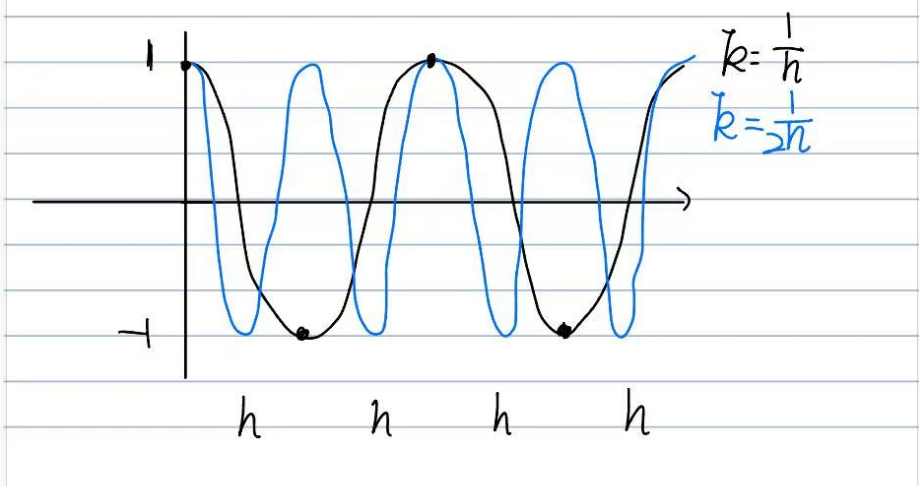
\includegraphics[width=0.3\textwidth]{p1.png}
\end{figure}

同理若给出边界条件0,则黑色$k= \frac{1}{h}$无法反映函数性质，当波峰在网格点上时，即蓝色$k = \frac{2}{3h}$.
\begin{figure}[H]
    \centering
    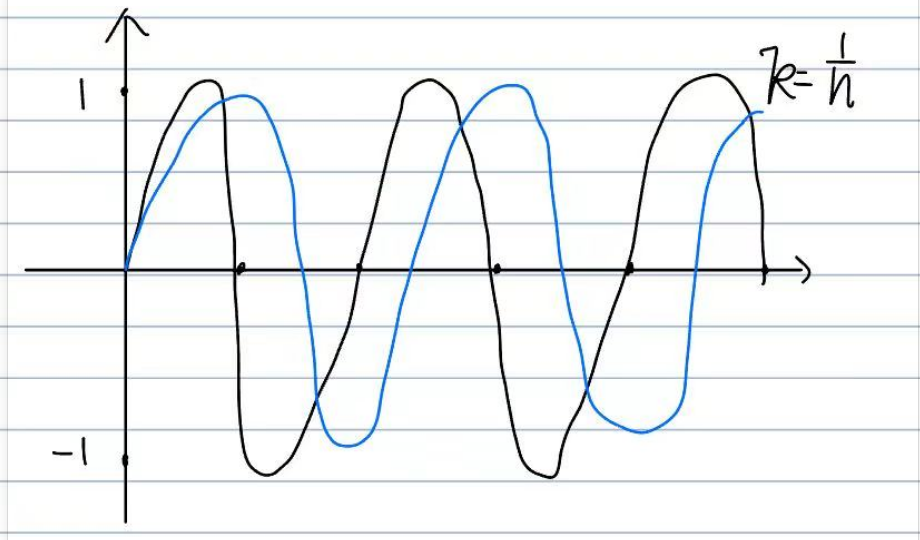
\includegraphics[width=0.3\textwidth]{p2.png}
\end{figure}


\subsection*{Exercise 9.17}
因为$T_w = I - \frac{wh^2}{2}A,$又因为已知$\lambda _k(A) = 4n^2 Sin^2 \frac{k\pi}{2n}, k=1,2,\cdots,n-1$,其中$ n = \frac{1}{h}$，

所以$\lambda _k (T_w) = \lambda _k (I) - \frac{wh^2}{2}\lambda _(A) = 1 - 2wSin^2 \frac{k\pi}{2n}$,

因为A对称正定，所以存在正交矩阵$Q, Q^T = Q^{-1}, Q^TAQ = diag\{\lambda_1(A), \lambda_2(A), \cdots, \lambda_{n-1}(A)\}$,

$\Rightarrow Q^TT_wQ = Q^T(I-\frac{wh^2}{2}A)Q = diag\{1-2wSin^2 \frac{pi}{2n}, \cdots, 1-2wSin^2 \frac{(n-1)pi}{2n}\} = diag\{\lambda_1(T_w), \cdots, \lambda_{n-1}(T_w)\}$.

这说明Q也是$T_w$的特征向量矩阵。

\subsection*{Exercise 9.35}
根据图Figure9.3,虚线的复杂度即为一个V-cirlce的复杂度，$2WU\sum_{k = 0}^{m} 2^{-kD} $,若在加上实线复杂度为：
\begin{align}
    2WU\sum_{k = 0}^{m} \sum_{i = m-k}^{m} 2^{-iD} &= 2WU\sum_{k=0}^{m} 2^{-(m-k)D}(\frac{1-2^{-(k+1)D}}{1-2^{-D}}) \\
                                &= 2WU\frac{1}{1-2^{-D}} \sum_{k=0}^{m} (2^{-(m-k)D} - 2^{-(m+1)D}) \\
                                &= 2WU\frac{1}{1-2^{-D}} (2^{-mD}\times \frac{1-2^{(m+1)D}}{1-2^{-D}} - (m+1)2^{-(m+1)D}) \\
                                &= 2WU\frac{1}{1-2^{-D}} (\frac{2^{-mD} - 2^D}{1-2^D} - (m+1)2^{-(m+1)D}) \\
                                &= 2WU\frac{1}{1-2^{-D}} (\frac{2^{-(m+1)D} - 1}{-2^{-D} -1} - (m+1)2^{-(m+1)D}) \\
                                &\leq \frac{2WU}{(1-2^{-D})^2}
\end{align}
所以$D=1:8WU;\  D=2:\frac{7}{2}WU;\ D=3:\frac{5}{2}WU$.

\subsection*{Exercise 9.41}
因为经过two-grid correction后，不论高频或是低频的残差都会被抑制，所以ci们的模长都会很小。

\subsection*{Exercise 9.45}
$I_h^{2h}:\mathbb{R} ^{n-1} \rightarrow \mathbb{R}^{\frac{n}{2}-1}$, 且$dimR(I_h^{2h})=rank(I_h^{2h}), dimN(I_h^{2h}) = n-1-dimR(I_h^{2h})$,

又因为已知$I_h^{2h }=$$\begin{pmatrix}
    1 & 2 & 1 & & & \\
      & 1 & 2 & 1 & \\
      & & 1 & 2 & 1 \\
       & &\cdot &\cdot &\cdot & \\
      & & & 1 & 2 & 1 \\
\end{pmatrix}$
是列满秩的，所以$dimR(I_h^{2h}) = \frac{n}{2} - 1, dimN(I_h^{2h}) = \frac{n}{2}$.







% ===============================================

\end{document}